\section{Tool screenshots}
\label{sect:tool-screenshots}

\begin{figure}[ht]
\centering
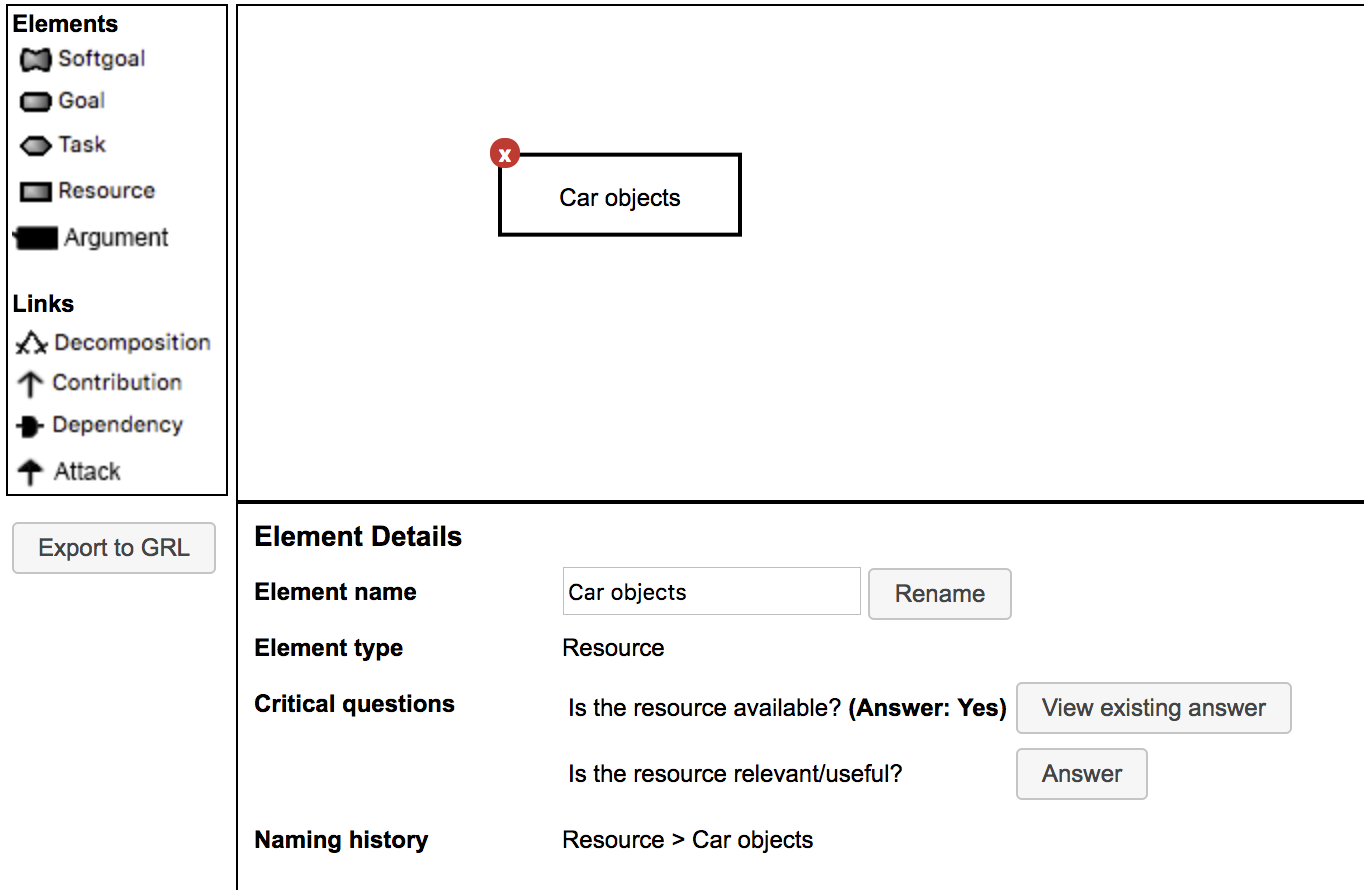
\includegraphics[scale=0.6]{img/tool-overview}
\caption{Overview of the RationalGRL tool}
\label{fig:tool:overview}
\end{figure}

\begin{figure}[ht]
\centering
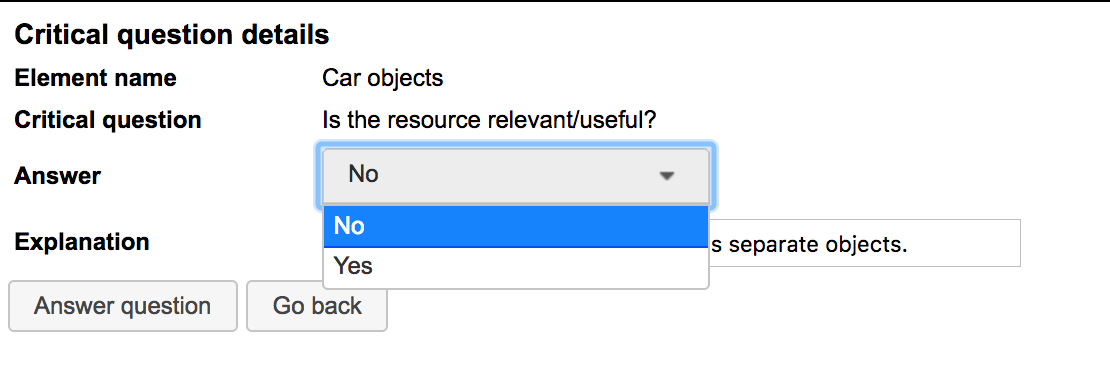
\includegraphics[scale=0.6]{img/tool-cqdetails}
\caption{Critical question details pane for ``Is the resource relevant/useful?''}
\label{fig:tool:cqdetails}
\end{figure}

\newpage

\begin{figure}[ht]
\centering
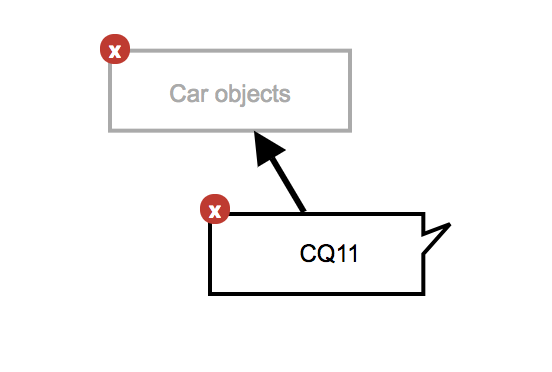
\includegraphics[scale=0.6]{img/tool-cqeffect}
\caption{Effect of answering CQ11: ``Is the resource reelevant/useful?'' with ``No''}
\label{fig:tool:cqeffect}
\end{figure}

\begin{figure}[ht]
\centering
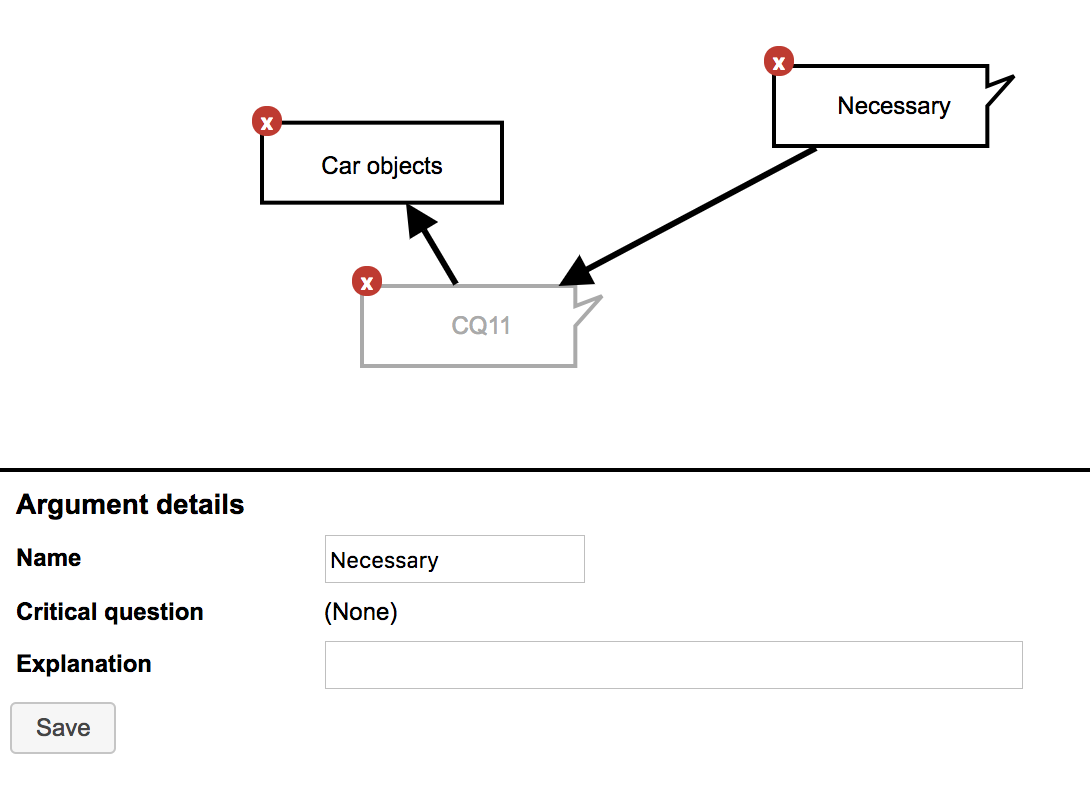
\includegraphics[scale=0.5]{img/tool-argument}
\caption{Argument details pane for generic argument ``Necessary''}
\label{fig:tool:argument}
\end{figure}

\begin{figure}[ht]
\centering
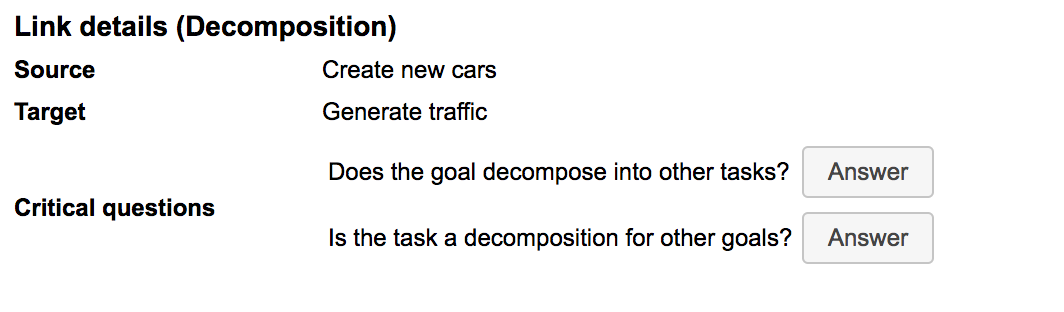
\includegraphics[scale=0.5]{img/tool-linkdetails}
\caption{Link details pane for decomposition link}
\label{fig:tool:cqdetails}
\end{figure}

\newpage

\begin{figure}[ht]
\centering
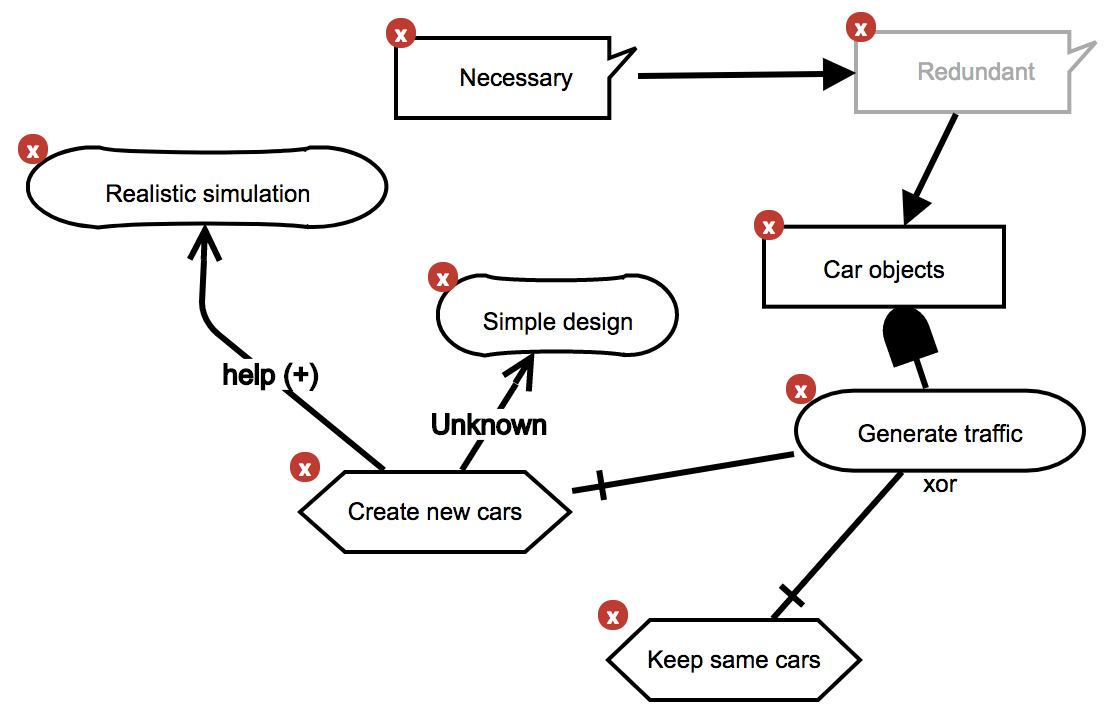
\includegraphics[scale=0.6]{img/tool-figfrompaper}
\caption{RationalGRL model of Figure~\ref{fig:example-small2} in the tool}
\label{fig:tool:figfrompaper}
\end{figure}

\begin{figure}[ht]
\centering
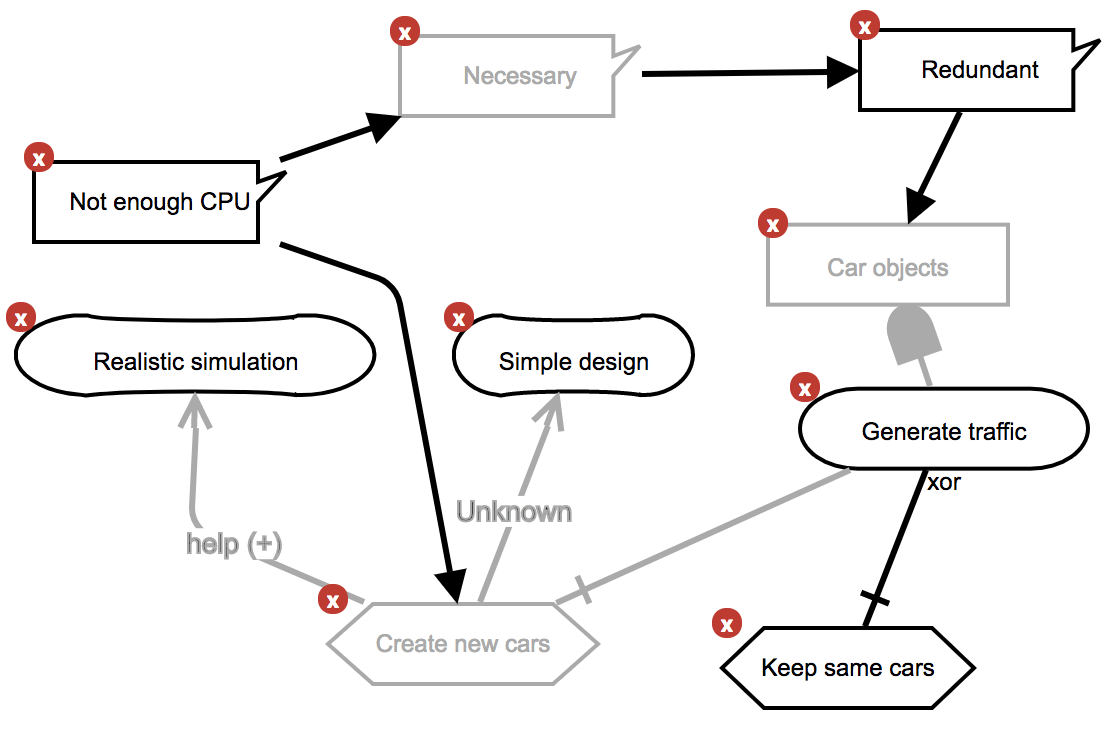
\includegraphics[scale=0.6]{img/tool-multipleattack}
\caption{Adding argument attack multiple arguments to Figure~\ref{fig:tool:figfrompaper}}
\label{fig:tool:multipleattack}
\end{figure}